%============================================================================
\documentclass[letterpaper, 11pt]{article}
\usepackage{comment} % enables the use of multi-line comments (\ifx \fi) 
\usepackage{lipsum} % generates Lorem Ipsum filler text. 
\usepackage{fullpage} % changes the margin
\usepackage{graphicx} % allows insertion of images

% tight center environment
\newenvironment{tightcenter}{\setlength\topsep{0pt}\setlength\parskip{0pt}
  \begin{center}
}{%
  \end{center}
}

%Custom Commands
\newcommand{\hl}{\begin{center} \line(1,0){475} \end{center}} % lines
\newcommand{\ctitle}[1]{\begin{center} \LARGE{#1} \end{center}} % custom title
\newcounter{fignum} \stepcounter{fignum} % counter for figure captions
\newcommand{\ecap}[1]{\begin{tightcenter} Figure \arabic{fignum}: {#1} \end{tightcenter} \stepcounter{fignum}} % easy caption
%============================================================================

% EE 16B FINAL PROJECT REPORT TEMPLATE, SPRING 2018
%	Based on the ECE 100 template by Patrick Bartman.
%	Edited by Mia Mirkovic and Dinesh Parimi.
%
% INSTRUCTIONS: Replace all the \lipsum with your text and delete all <> and 
% examples/placeholders/fillers when finished. If you use external sources, 
% make sure to include them in the References section and cite them with the 
% \cite command as demonstrated. The rest should be self-explanatory. GLHF!

\begin{document}

%Header 
\noindent
EE 16B Spring 2018 \hfill  \textless Student1 Name\textgreater: ee16b-\textless login1\textgreater \\
\normalsize Profs. Roychowdhury and Maharbiz \hfill \textless Student2 Name\textgreater: ee16b-\textless login2\textgreater \\

%Title

\ctitle{SIXT33N Project Report}


\hl
\section*{Circuit}
\subsection*{Final Design}
% citation example!
Example of a Citation\cite[p.219]{Robotics}. Here's another citation\cite{Flueck}. 

\noindent \lipsum[1]

\subsection*{Gain and Frequency Response}
\lipsum[2]
\hl 

\section*{PCA Classification}
\subsection*{Commands}
\lipsum[3]

\subsection*{Processing}
\lipsum[4]
\hl 

\section*{Controls}
\subsection*{Open Loop Model}
\lipsum[5]

\subsection*{Closed Loop Model}
\lipsum[6]

\subsection*{Choosing Controller Values}
\lipsum[7]

\subsection*{General Comments}
\lipsum[8]
\hl 


\section*{Video}
% Uncomment the line below and input your URL.
%\url{YOUR URL HERE}
\hl 

\section*{Figures}
% Replace "ckt" and "block" with your images.
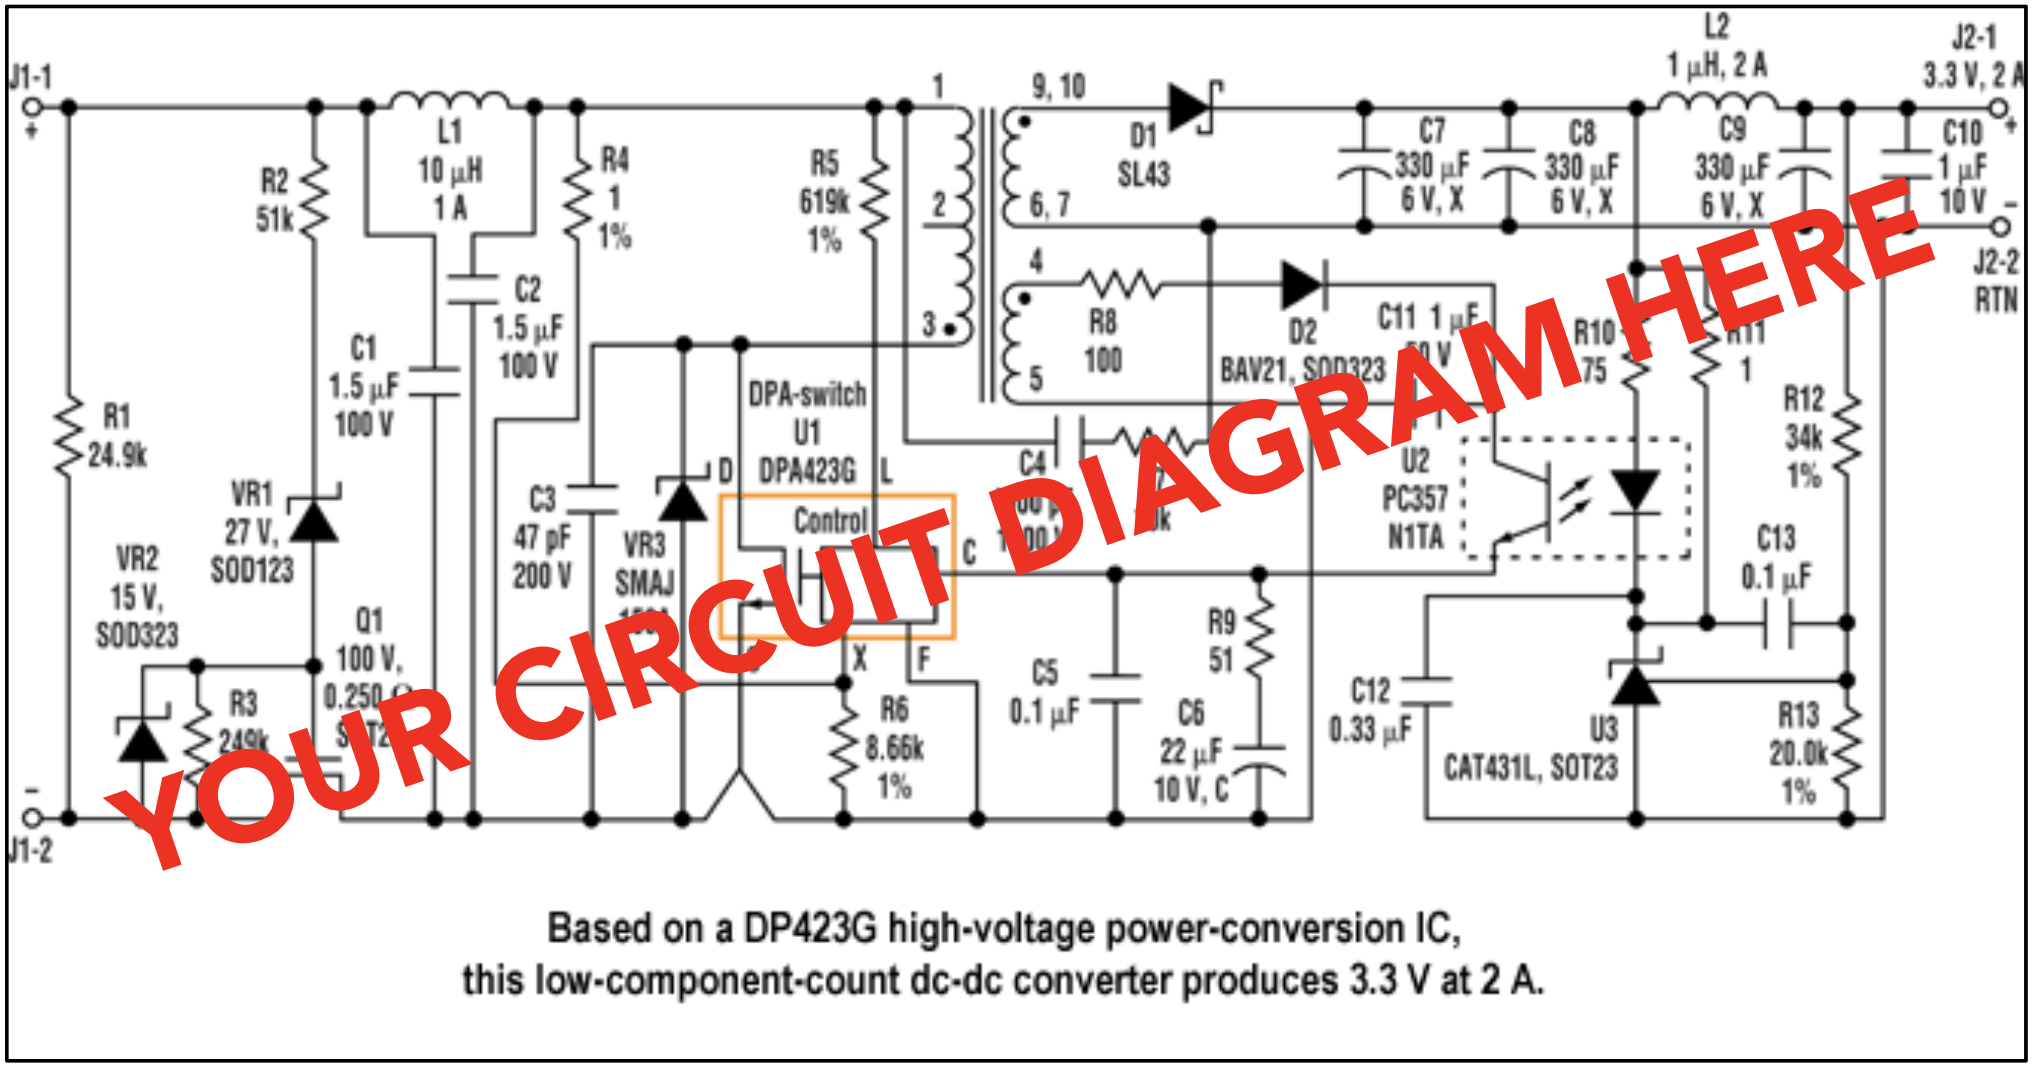
\includegraphics[width=\textwidth]{ckt}
\ecap{Full Circuit Diagram}

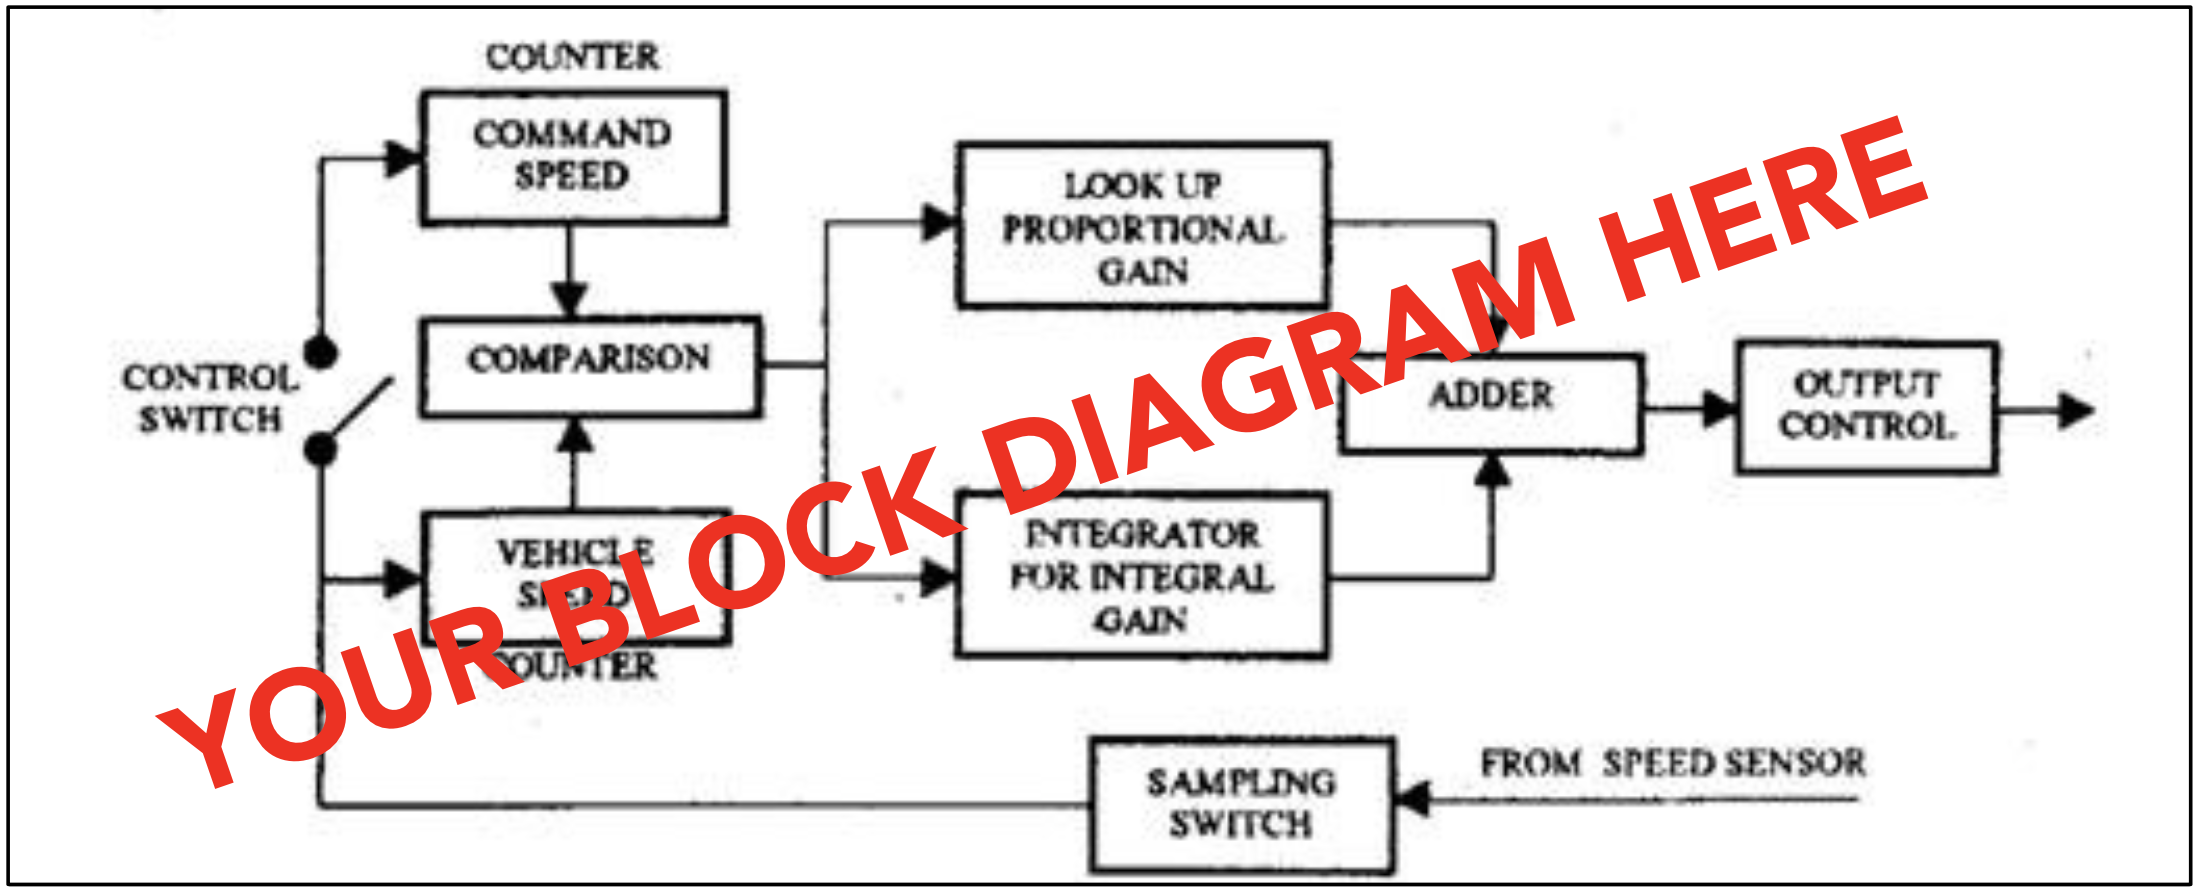
\includegraphics[width=\textwidth]{block}
\ecap{Closed Loop Control Scheme Block Diagram}

\hl

\begin{thebibliography}{9}
% DON'T FORGET TO REPLACE WITH YOUR REFERENCES!
\bibitem{Robotics} Fred G. Martin \emph{Robotics Explorations: A Hands-On Introduction to Engineering}. New Jersey: Prentice Hall.
\bibitem{Flueck}  Flueck, Alexander J. 2005. \emph{ECE 100}[online]. Chicago: Illinois Institute of Technology, Electrical and Computer Engineering Department, 2005 [cited 30
August 2005]. Available from World Wide Web: (http://www.ece.iit.edu/~flueck/ece100).
\end{thebibliography}

\end{document}
